
% --- Configuración de Listings para Código Python ---
\definecolor{codegreen}{rgb}{0,0.6,0}
\definecolor{codegray}{rgb}{0.5,0.5,0.5}
\definecolor{codepurple}{rgb}{0.58,0,0.82}
\definecolor{backcolour}{rgb}{0.95,0.95,0.92}

\lstdefinestyle{mystyle}{
    backgroundcolor=\color{backcolour},
    commentstyle=\color{codegreen},
    keywordstyle=\color{magenta},
    numberstyle=\tiny\color{codegray},
    stringstyle=\color{codepurple},
    basicstyle=\footnotesize\ttfamily, % Fuente monoespaciada pequeña
    breakatwhitespace=false,
    breaklines=true,
    captionpos=b,
    keepspaces=true,
    numbers=left,
    numbersep=5pt,
    showspaces=false,
    showstringspaces=false,
    showtabs=false,
    tabsize=2,
    language=Python % Especifica el lenguaje
}
\lstset{style=mystyle} % Aplica el estilo por defecto

% --- Configuración de Hyperref ---
\hypersetup{
    colorlinks=true,
    linkcolor=blue,
    filecolor=magenta,
    urlcolor=cyan,
    pdftitle={Informe TP1 - Antenas y Propagación},
    pdfpagemode=FullScreen,
}

\section{Introducción}
% =============================================
El presente trabajo práctico tiene como objetivo analizar las características fundamentales de las antenas dipolo de alambre fino. Se estudiará cómo varían sus parámetros principales, como el patrón de radiación, la resistencia de radiación, la directividad y la apertura efectiva, en función de la longitud eléctrica del dipolo (L/$\lambda$).

Para llevar a cabo este análisis, se utilizaron herramientas de programación en Python, aprovechando bibliotecas como NumPy para cálculos numéricos, Matplotlib para la generación de gráficos 2D y 3D estáticos, y opcionalmente Mayavi y PyVista para visualizaciones 3D más avanzadas o interactivas.

Se implementaron las fórmulas teóricas correspondientes a cada parámetro y se generaron gráficos para visualizar su comportamiento. Los resultados obtenidos permitirán comprender mejor el funcionamiento de este tipo de antenas, que son fundamentales en muchas aplicaciones de radiocomunicaciones.
\section*{Desarrollo}
% =============================================
\section{Ejercicio 1: Patrones de Radiación}
% =============================================
Este ejercicio consiste en graficar y analizar el patrón de radiación normalizado en amplitud, $|F(\theta)|$, para un dipolo de longitud L ubicado simétricamente respecto al origen y orientado según el eje z. Se consideran tres longitudes eléctricas específicas: L = $\lambda$/2, L = $\lambda$ y L = 1.5$\lambda$.


La expresión del campo radiado por un dipolo ideal está dada por:

\[
\hat{E}_\theta = \frac{j \eta_0 I}{2\pi r} e^{-j\beta_0 r} \left[ \frac{\cos\left(\frac{\beta_0 L}{2} \cos\theta\right) - \cos\left(\frac{\beta_0 L}{2}\right)}{\sin\theta} \right]
\]

Donde $\beta_0 = \frac{2\pi}{\lambda}$ es el número de onda, $L$ la longitud del dipolo y $\theta$ el ángulo de observación.

\subsubsection*{Repositorio del proyecto}

Todo el código fuente, imágenes generadas y documentación relacionada con este trabajo práctico se encuentra disponible en el siguiente repositorio de GitHub:

\begin{center}
\texttt{https://github.com/GenaroTrucchi/Antenas-PropdeOndas.git}
\end{center}

Allí se pueden encontrar los scripts en Python utilizados para generar las figuras, el entorno virtual con las dependencias necesarias, así como también este informe en formato \LaTeX{}.

Para ejecutar el proyecto localmente, puede seguirse el procedimiento detallado en el archivo \texttt{README.md} incluido en el repositorio.
A continuacion se muestran lo resultados obtenidos:

% Lista de longitudes relativas
\def\relativelengths{{0.12},{0.25},{0.50},{0.75},{1.25},{1.50},{1.75},{2.00},{2.25}}

\newcommand{\incluirImagenes}[1]{
  \begin{figure}
    \centering
    \begin{subfigure}[b]{0.45\textwidth}
        \includegraphics[width=\textwidth]{Imagenes2D/2D_Lrel_#1.png}
        \caption{Gráfico 2D}
    \end{subfigure}
    \begin{subfigure}[b]{0.45\textwidth}
        \includegraphics[width=\textwidth]{Imagenes3D/3D_Lrel_#1.png}
        \caption{Gráfico 3D}
    \end{subfigure}
    \caption{Patrón de radiación para $L/\lambda = #1$}
  \end{figure}
}

% Incluir todas las imágenes
\incluirImagenes{0.12}
\incluirImagenes{0.25}
\incluirImagenes{0.50}
\incluirImagenes{0.75}
\incluirImagenes{1.25}
\incluirImagenes{1.50}
\incluirImagenes{1.75}
\incluirImagenes{2.00}
\incluirImagenes{2.25}

Ademas que se realizo un seccion en donde se pueden ver en 3D lasgraficas con la ayuda de la Herramienta "PyVita
Acontinuacion ejemplos 
  \begin{figure}
    \centering
    \begin{subfigure}[b]{0.45\textwidth}
        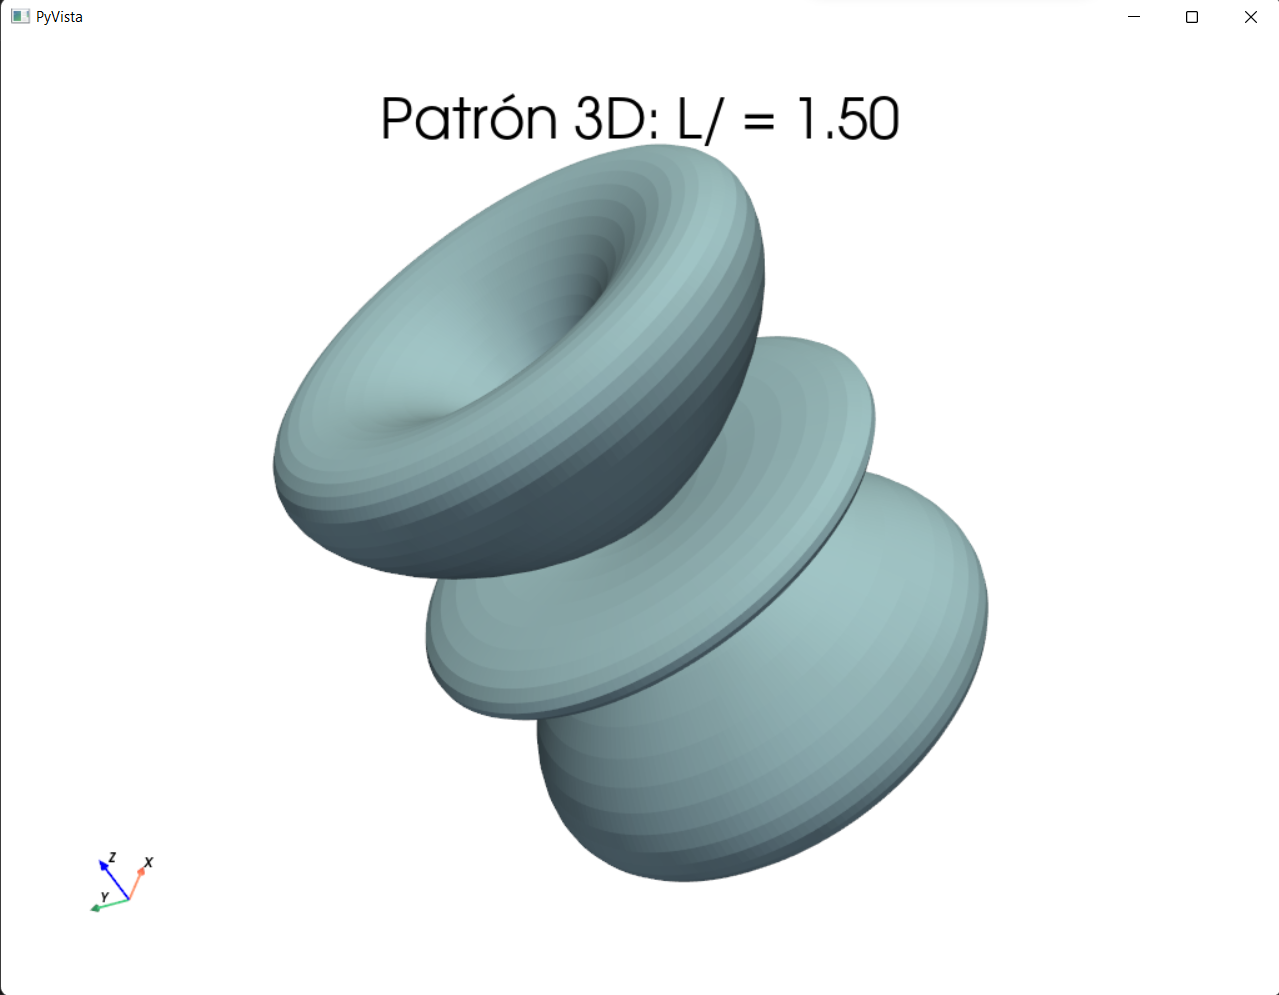
\includegraphics[width=\textwidth]{Imagenes3D/Vita1.png}
        \caption{Gráfico 2D}
    \end{subfigure}
    \begin{subfigure}[b]{0.45\textwidth}
        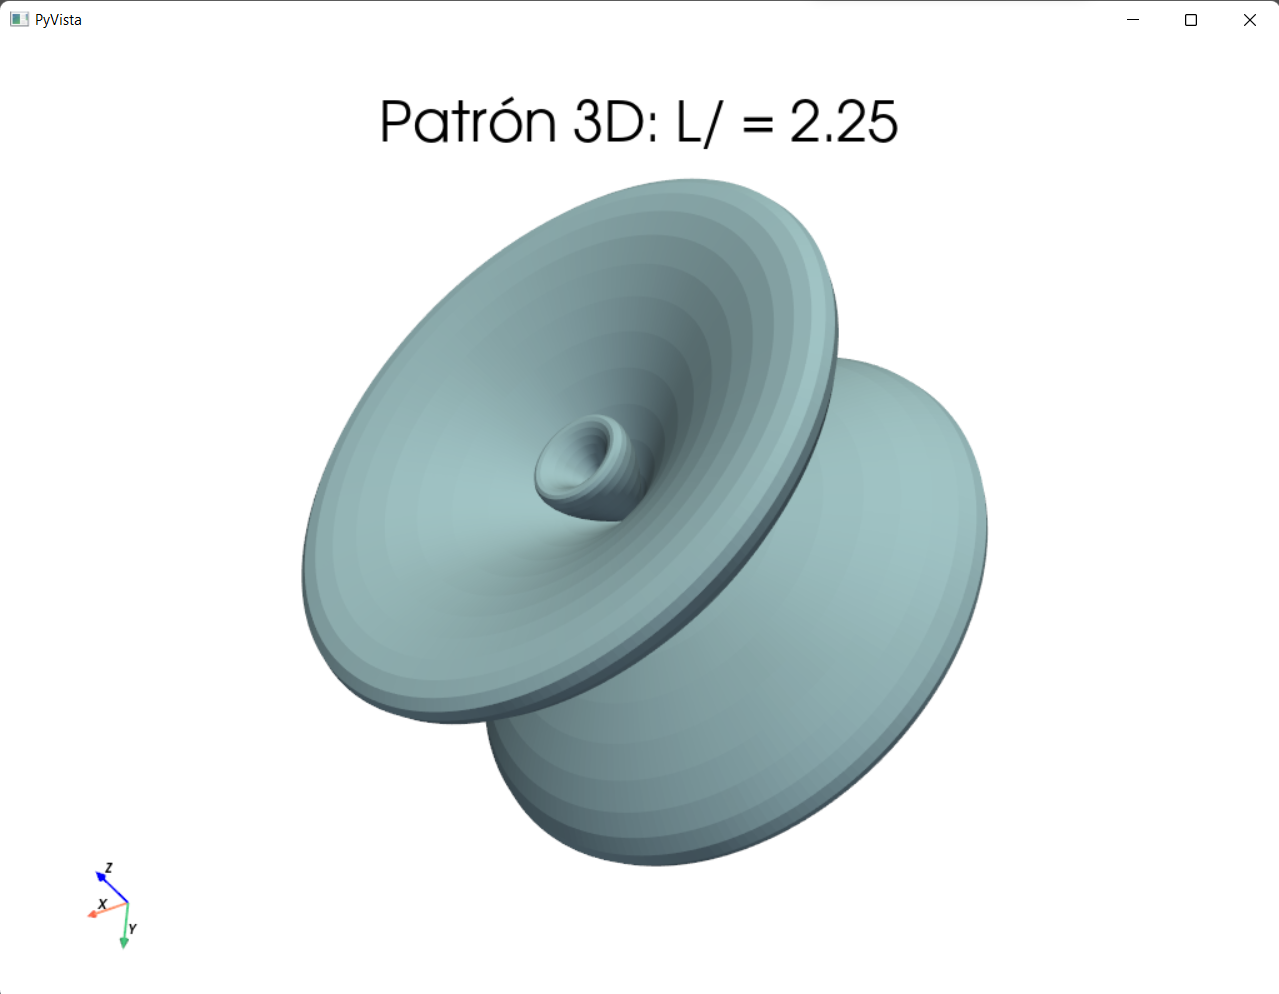
\includegraphics[width=\textwidth]{Imagenes3D/Vita_2.png}
        \caption{Gráfico 3D}
    \end{subfigure}
  \end{figure}

\section*{Conclusión}
Se observó cómo al aumentar la longitud relativa del dipolo ($L/\lambda$) aparecen lóbulos secundarios en el patrón de radiación. Por esta razón, se prefiere mantener longitudes menores o iguales a $\lambda/2$ para una emisión más direccional y con menor interferencia.



